\newcommand{\econtexRoot}{.}
% The \commands below are required to allow sharing of the same base code via Github between TeXLive on a local machine and ShareLaTeX.  This is an ugly solution to the requirement that custom LaTeX packages be accessible, and that ShareLaTeX seems to ignore symbolic links (even if they are relative links to valid locations)
\providecommand{\econtex}{\econtexRoot/texmf-local/tex/latex/econtex}
\providecommand{\econtexSetup}{\econtexRoot/texmf-local/tex/latex/econtexSetup}
\providecommand{\econtexShortcuts}{\econtexRoot/texmf-local/tex/latex/econtexShortcuts}
\providecommand{\econtexBibMake}{\econtexRoot/texmf-local/tex/latex/econtexBibMake}
\providecommand{\econtexBibStyle}{\econtexRoot/texmf-local/bibtex/bst/econtex}
\providecommand{\notes}{\econtexRoot/texmf-local/tex/latex/handout}
\providecommand{\handoutSetup}{\econtexRoot/texmf-local/tex/latex/handoutSetup}
\providecommand{\handoutShortcuts}{\econtexRoot/texmf-local/tex/latex/handoutShortcuts}
\providecommand{\handoutBibMake}{\econtexRoot/texmf-local/tex/latex/handoutBibMake}
\providecommand{\handoutBibStyle}{\econtexRoot/texmf-local/bibtex/bst/handout}

  

\documentclass{beamer}
\usepackage{etoolbox}
\usepackage{comment}
\usepackage{graphicx}
%\usepackage{dtklogos}
\usepackage{dsfont}
\usepackage{amsmath,amssymb}
\usepackage{\econtexShortcuts}
\usepackage[english]{babel}
\usepackage[svgnames,hyperref]{}
\usepackage{empheq}
\usepackage[many]{tcolorbox}
\usepackage{remreset}
\usepackage{tikz} 
\usetikzlibrary{tikzmark,fit,shapes.geometric}
\usetikzlibrary{tikzmark,calc,arrows,shapes,decorations.pathreplacing}
\tikzset{every picture/.style={remember picture}}
\usepackage{cancel}
\usepackage{booktabs,natbib}
\setbeamercovered{invisible}

\usepackage{dcolumn}

\tcbset{highlight math style={enhanced,
		colframe=red!60!black,colback=yellow!50!white,arc=4pt,boxrule=1pt,
}}


\makeatletter
\@removefromreset{subsection}{section}
\patchcmd{\beamer@part}{\setcounter{subsection}{0}}{}{}
\makeatother
\setcounter{subsection}{1}
\setbeamercovered{transparent}
\setbeamertemplate{navigation symbols}{}%remove navigation symbols
\begin{comment}
\setbeamertemplate{footline}
{
	\hbox{\begin{beamercolorbox}[wd=1\paperwidth,ht=2.25ex,dp=1ex,right]{framenumber}%
			\usebeamerfont{framenumber}\insertframenumber{} \hspace*{2ex}
	\end{beamercolorbox}}%
	\vskip0pt%
}
\end{comment}


\mode<presentation>{}
%% preamble
\title[Who Pays Attention to Euler?]{Who Pays Attention to Euler?}
\author{Edmund Crawley and Fabian Winkler}
%\date[03/05/2020]{March, 2020}
\date[03/05/2020]{}
\usetheme{Frankfurt}

\setbeamertemplate{navigation symbols}{}
\makeatletter
\setbeamertemplate{footline}
{%
	\hbox{\begin{beamercolorbox}[wd=1\paperwidth,ht=2.25ex,dp=1ex,right]{framenumber}%
		\usebeamerfont{framenumber}\insertframenumber{} \hspace*{2ex}
	\end{beamercolorbox}}%
	\vskip0pt%
	\pgfuseshading{beamer@barshade}%
	\ifbeamer@sb@subsection%
	\vskip-9.75ex%
	\else%
	\vskip-7ex%
	\fi%
	\begin{beamercolorbox}[ignorebg,ht=2.25ex,dp=3.75ex]{section in head/foot}
		\insertnavigation{\paperwidth}
	\end{beamercolorbox}%
	\ifbeamer@sb@subsection%
	\begin{beamercolorbox}[ignorebg,ht=2.125ex,dp=1.125ex,%
		leftskip=.3cm,rightskip=.3cm plus1fil]{subsection in head/foot}
		\usebeamerfont{subsection in head/foot}\insertsubsectionhead \insertframenumber{} \hspace*{2ex}
	\end{beamercolorbox}%
	\fi%
}%
\setbeamertemplate{headline}{%
}
\makeatother
\begin{document}
\setbeamertemplate{caption}{\raggedright\insertcaption\par}
\newcolumntype{d}[1]{D{.}{.}{#1}}
%circled draws a circle around a number
\newcommand*\circled[1]{\tikz[baseline=(char.base)]{
		\node[shape=circle,draw,inner sep=2pt] (char) {#1};}}

\begin{frame}[plain]
\titlepage
\end{frame}
\addtocounter{framenumber}{-1}
\section{Introduction}
\setbeamercovered{invisible}
\frame{
\frametitle{Mortgages and monetary policy transmission}
\begin{itemize}
\item In partial equilibrium models, mortgages play an important role in monetary policy transmission\\
e.g. \cite{wong_population_2016}, \cite{berger_prepayment_2018}, \cite{eichenbaum_refinance_2018}\pause
\item BUT in general equilibrium monetary policy doesn't move long real rates by much, so mortgages do not play a role\\
e.g \cite{greenwald_mortgage_2018}, \cite{garriga_monk_2019}\pause
\end{itemize}
 This tension in the literature has to do with intertemporal substitution.
}

\frame{
	\frametitle{The Euler Equation}
	$u'(c_t) = \beta R_{t+1} \mathbb{E}u'(c_{t+1})$ \\
\pause
\bigskip
Partial equilibrium example: Real rate goes up 1\% for one year\\
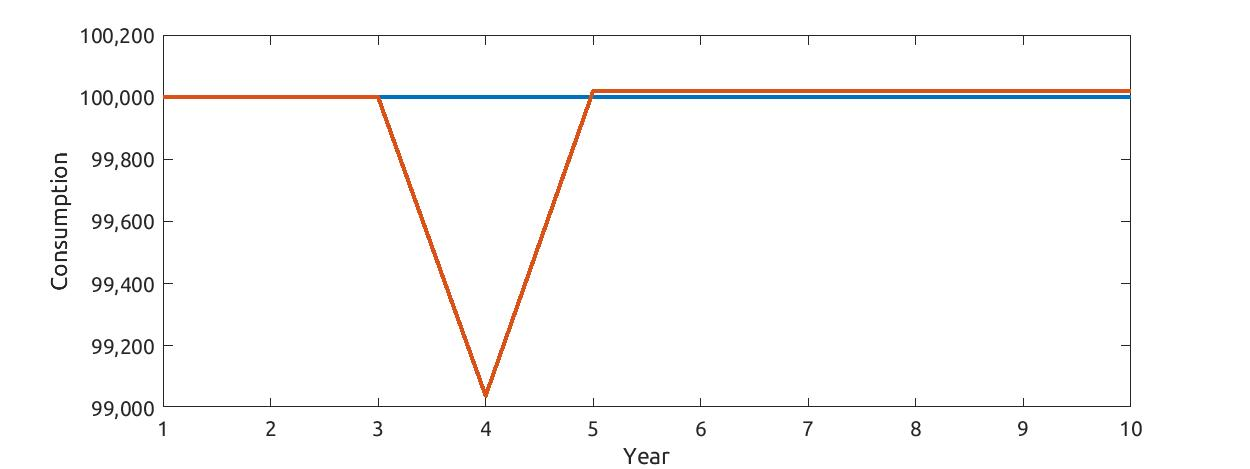
\includegraphics[width=0.9\textwidth]{../../Code/Dynare/Figures/MotivatingExample.jpg}\\
Consumption of a HH with \$100k annual income goes down nearly \$500 (IES = 0.5) \\
\pause
\bigskip
BUT: This change in behavior is worth just \$2.50 to the household\\
\bigskip
Canonical monetary policy models work via an incentive that is worth less than a cup of coffee
}

\frame{
\frametitle{Evidence for Intertemporal Substitution}
\begin{itemize}
\item Macro: Complete failure of relation between real rates and consumption growth
\item Micro: No convincing evidence interest rate incentives incite intertemporal substitution
\item 30-year treasury down almost 2 percentage points since Nov 2018 $\implies$ I should increase consumption by over 10\% today (all else equal)
\item When I ask financial advisors how interest rates change their saving advice, they look at me like I'm crazy!
\item Evidence from default pension saving: people really don't pay attention to this decision - \cite{madrian_power_2001}
\end{itemize}
}

\frame
{
	\frametitle{Interest Rates: For Whom is Inattention Costly?}
	Main Idea:
	\begin{itemize}
		\item Entirely rational for unconstrained households to ignore interest rates 
		\item Constrained agents \textit{cannot} ignore interest rates: they directly determine constraints
		\item Mortgage refinancing decisions are not ignored
	\end{itemize}
	\pause
	\bigskip
	We examine a Two Agent New Keynesian (TANK) model in which
	\begin{itemize}
		\item Unconstrained agents are inattentive
		\item Constrained agents are attentive
		\item Refinancing decisions are made \`a la \cite{greenwald_mortgage_2018}
	\end{itemize}
}
\frame{
\frametitle{Implications}
Puzzles resolved:
\begin{itemize}
	\item Monetary policy affects long term real rates
	\item Mortgages matter for policy transmission
	\item Forward Guidance puzzle disappears ($\approx$ Euler eq. discounting)
\end{itemize}
\bigskip
Policy Implications:
\begin{itemize}
%FW: These two bullets are still a bit mysterious to me
	\item Monetary Policy acts through redistribution (and investment)
	\item Much closer relation to fiscal policy
\end{itemize}
}

\section{Costs of Inattention}
\begin{comment}
\frame{
\frametitle{Costs of Inattention: A Two-Period Example}
Consider a two period model with consumer maximizing:
\begin{align*}
\log(C_1) +  \log(C_2)
\end{align*}
$R=1$ and income $Y_1 = Y_2 = Y$. Solution is $C_1 = C_2 = Y$
\pause
\bigskip
Now $R$ is increased to $1+r$. (Linearized) Solution is:
\begin{align*}
C_1 = (1-\frac{r}{2  }) Y\\
C_2 = (1+\frac{r}{2 }) Y 
\end{align*}
\pause
\bigskip
Suppose you didn't pay attention and consumed $C_1 = C_2 = Y$ as before. \textbf{Loss of utility would be second order.}
}
\frame{
\frametitle{Costs of Inattention: An Example with Refinancing}
\begin{itemize}
\item Now assume you start owing a debt of $D$ in period 2, with an offsetting income of $D$ in period 2.\\
\item You have the option to refinance at a face value of $D$.\\
\item Suppose debt is equal to income, $D=Y$\\
\end{itemize}
If $R$ goes up, you will not refinance - problem is identical to the above:
 \begin{align*}
 C_1 = (1-\frac{r}{2 }) Y\\
 C_2 = (1+\frac{r}{2}) Y 
 \end{align*}
However, if $R$ goes down, you can refinance and only pay $(1+r)D$ next period
 \begin{align*}
C_1 = (1-r) Y\\
C_2 =  Y
\end{align*}
If you didn't notice this, loss to utility would be \textbf{first order}.
}
\end{comment}
\frame{
\frametitle{Costs of Inattention: A Numerical Example}
Model:
\begin{itemize}
\item 40 years of life
\item Consumption and Income constant in baseline ($\beta= 1/R$)
\item Consumer has a mortgage, face value one year of income, fixed installments for 20 years.
\item Experiment: Shock real rate - exponentially decaying shock with half life 2.5 years (5 year rates moves 0.5x size of shock
\end{itemize}
\pause
\bigskip
What are the costs of in inattention to the interest rate shock with regards to:
\begin{itemize}
\item Intertemporal Substitution
\item Mortgage Refinancing
\end{itemize}
}
\frame{
\frametitle{Costs of Inattention: Intertemporal vs Refiancing}
\centering
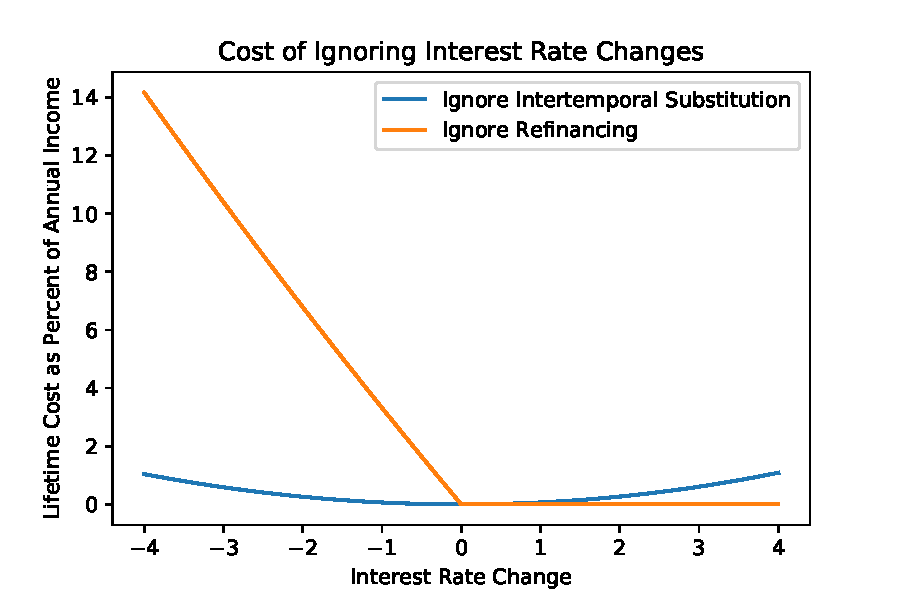
\includegraphics[width=\textwidth]{../../Code/HARK/Figures/CostofInattention.pdf}
}

\section{NK Model}
\frame{
\frametitle{A Two-Agent NK model with Debt}
Two agents:
\begin{itemize}
\item[1] Standard unconstrained, forward-looking agent
\item[2] Hand-to-mouth agent, able to borrow, subject to borrowing constraint on income
\end{itemize}
\bigskip
Shock to Taylor Rule is VERY persistent
}

\frame{
\frametitle{Impulse Responses to Persistent Monetary Shock}
Nominal Rate Moves in Opposite Directions
\centering
	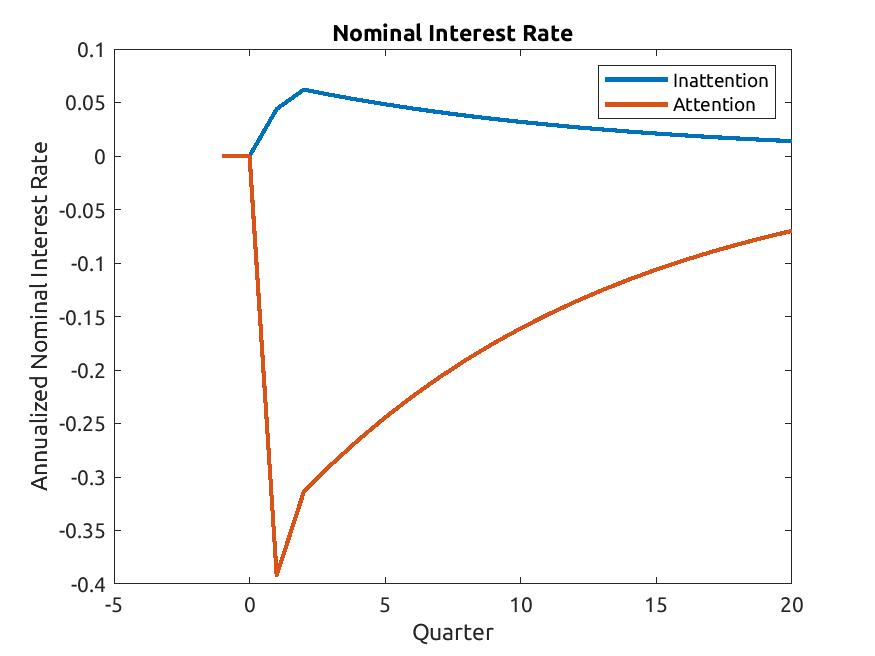
\includegraphics[width=0.9\textwidth]{../../Code/Dynare/Figures/NominalRate.jpg}
}
\frame{
\frametitle{Impulse Responses to Persistent Monetary Shock}
\centering
	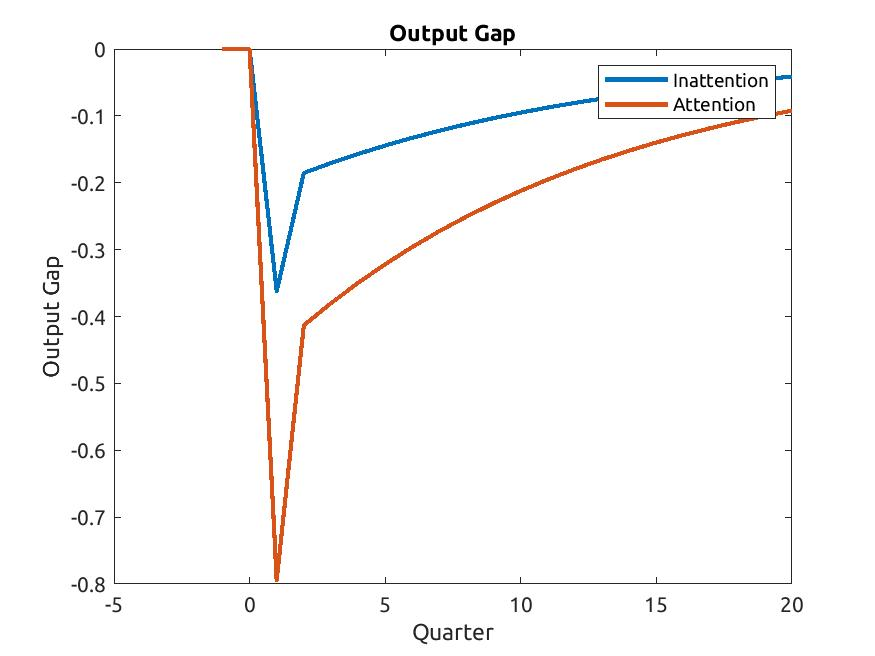
\includegraphics[width=0.45\textwidth]{../../Code/Dynare/Figures/OutputGap.jpg}
	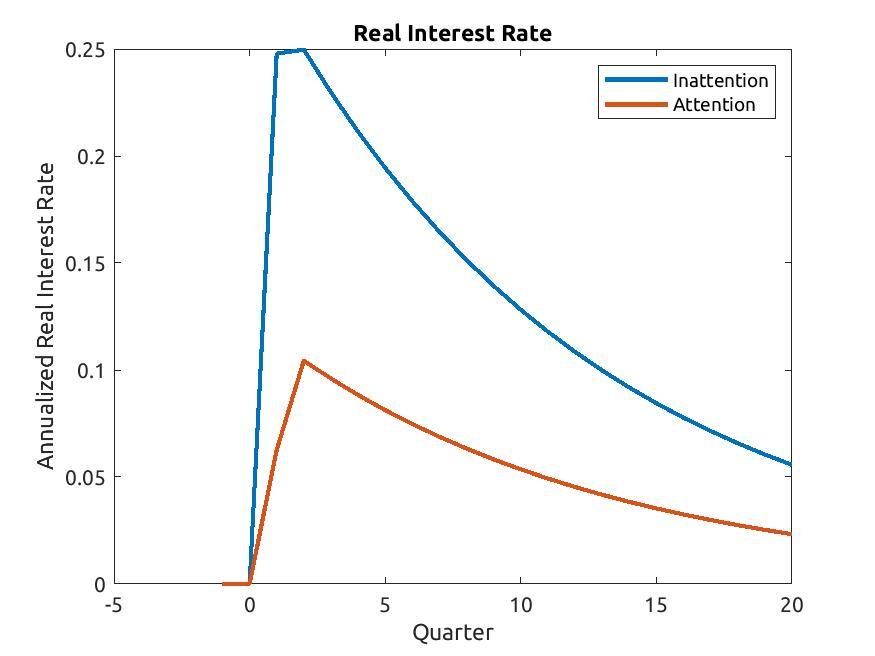
\includegraphics[width=0.45\textwidth]{../../Code/Dynare/Figures/RealRate.jpg}\\
	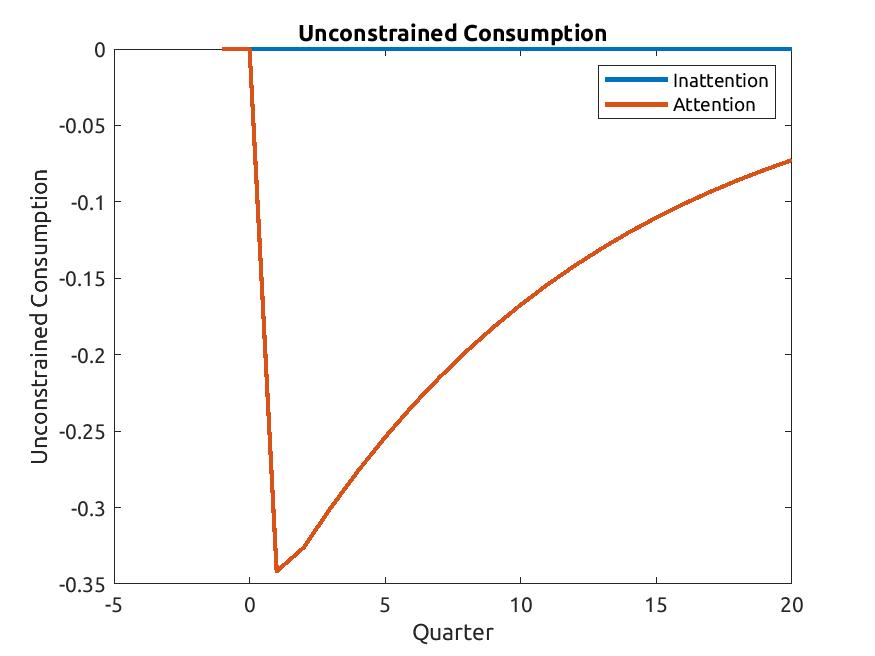
\includegraphics[width=0.45\textwidth]{../../Code/Dynare/Figures/UnconstrainedConsumption.jpg}
	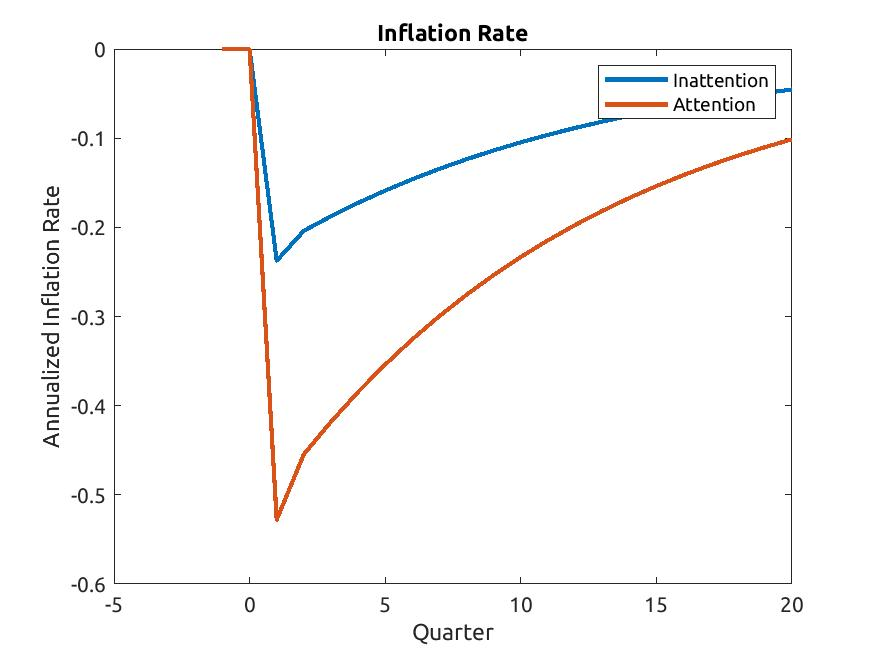
\includegraphics[width=0.45\textwidth]{../../Code/Dynare/Figures/Inflation.jpg}
}


\bibliographystyle{\econtexBibStyle}
\newsavebox\mytempbib
\savebox\mytempbib{\parbox{\textwidth}{\bibliography{\econtexRoot/WhoPaysAttention}}}


\end{document}


